\begin{figure}
\begin{center}
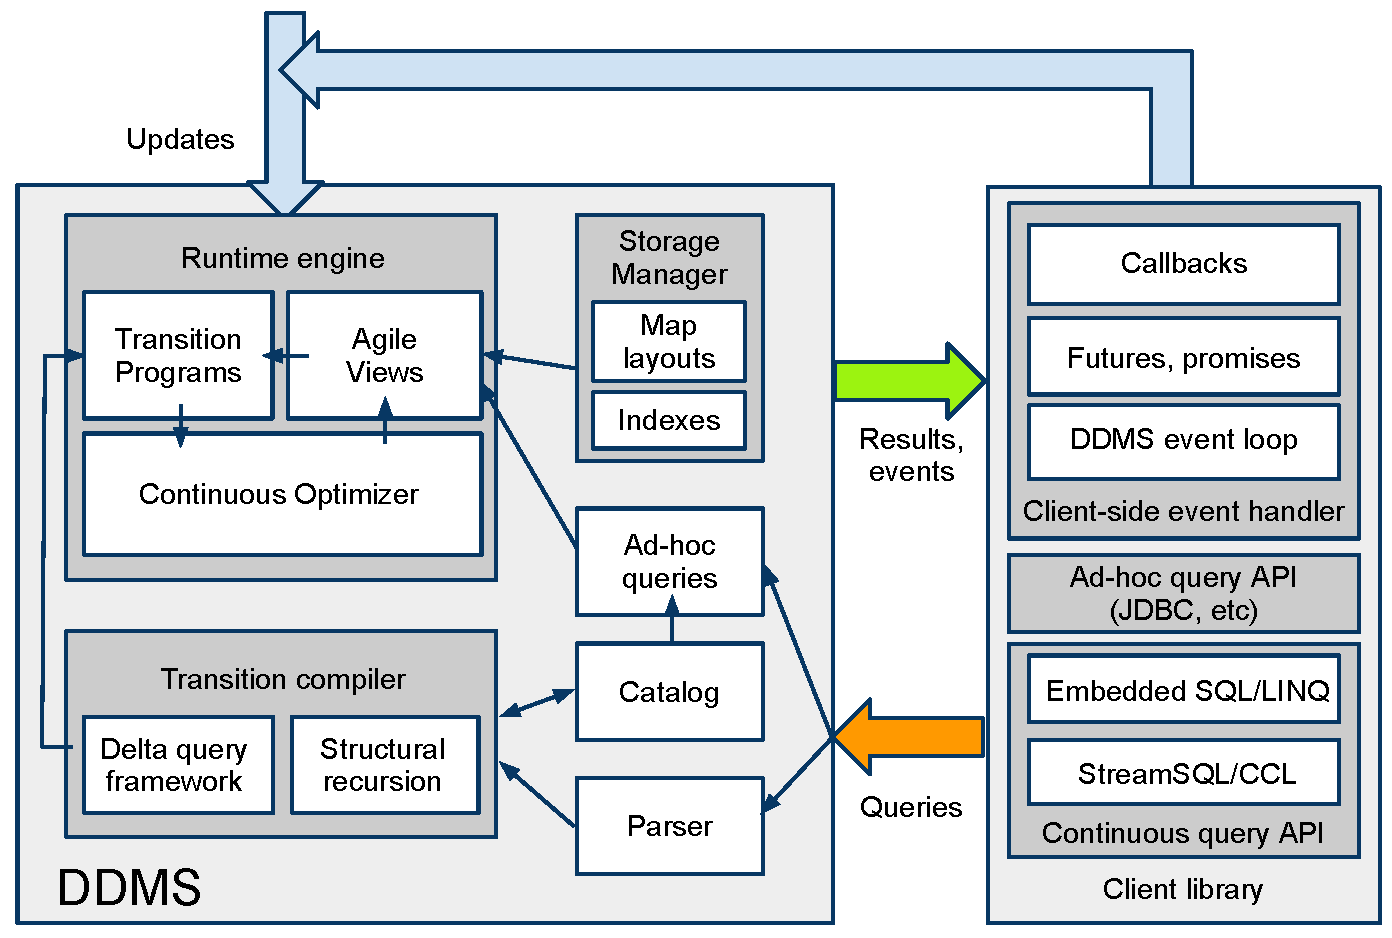
\includegraphics[width=3.3in]{graphics/CIDRarch.pdf}
\end{center}
\vspace*{-0.2in}
\caption{Dynamic Data Management System (DDMS) and Application Interface
Architecture}
\label{fig:ddmsarch}
\vspace*{-0.2in}
\end{figure}

We now examine the architecture of a DDMS, as illustrated in Figure
\ref{fig:ddmsarch}.  The core component of a DDMS is its runtime engine.  Unlike
a traditional database system where the same engine manages all database
instances, each individual DDMS execution runtime is constructed around a
specific set of queries provided by the client program (e.g., via SQL code
embedded inline in the program), each defining an \textit{agile view}.

\subsection{Application Interfaces}

The data that is processed by a DDMS arrives at the system in the form of an
update stream of tuple insertions, deletions and modifications. The stream need
not be ordered in any shape or form, and deletions are assumed to apply to
tuples that have already been seen at some arbitrary prior point on the stream.
Updates are fully processed on-the-fly, and their effects on agile views are
realised in atomic fashion, prior to working on any subsequent update. Depending
on the type of results requested by queries, any results arising from updates
will be directly forwarded to application code as agile views are maintained.

DBToaster provides a wide variety of client interfaces to issue queries and
obtain results from the DDMS, to reflect the diverse needs of applications built
on top of our tool. Today's stream processors tend to be black-box systems that
run completely decoupled from the application. Client libraries interact with
stream processors through remote procedure call abstractions, issuing queries
and new data through function calls, and either polling or being notified
whenever results appear on a queue that is associated with a TCP socket
connected to the stream processor.

In DBToaster, the set of agile views requested by clients, the \textit{visible
schema}, forms the primary read interface between client programs and the DDMS
runtime. Clients can submit queries for which the DDMS materializes an agile
view through three methods:
(1) a continuous query client API, as done with existing stream client
libraries, which sends a query string to the DDMS server for parsing,
compilation, and agile view construction. The query string may be specified in a
standard streaming language such as StreamSQL or CCL~\cite{jain-pvldb:08}. The
client may specify several ways to receive results, as seen below.
(2) an ad-hoc query client API, which issues a one-time query to the
DDMS, and returns the agile view as a datastructure to be used by the remainder
of the client program. This API may be used in both synchronous and
asynchronous modes, as indicated by the type of result requested. The query is
specified in standard SQL.
(3) an embedded language, whose syntax and data model are natural fits to the
host language in which the client application is written. Examples include
embedded SQL, and collection comprehension oriented approaches such as LINQ,
Links, and Ferry~\cite{meijer-sigmod:06,cooper-fmco:06,grust-sigmod:09}.
One interesting challenge with the embedded language approach is that of
enabling asynchronous event-driven programming. Whereas language embeddings
are natural for ad-hoc querying, we have yet to see these approaches
for stream processing.

Given these modes of issuing queries to the DDMS, our client interface supports
four methods of receiving results:
(1) callbacks, which can be specified as handlers as part of the continuous query
API. Callbacks receive a stream of query results, and are the simplest form of
result handlers that run to completion on query result events.  
(2) a DDMS event loop, which multiplexes result streams for multiple queries.
Applications may register callbacks to be executed on any result observed on the
event loop, allowing complex application behavior through dynamic
registration, observation and processing of results on the event loop.
(3) dynamic datastructures, which are read-only from the application
perspective. The datastructure appears as a native collection type in the host
language, facilitating natural access for the remainder of the program. Ad-hoc
queries use this method for results by default. Continuous queries may also use
this method in which case the datastructure acts as a proxy with accessors that
pull in any updates from the DDMS when invoked.
(4) promises and futures~\cite{Liskov:1988:PLS:53990.54016}, which provide a
push-based proxy datastructure for the
result. A future is an object whose value is not initially know and is provided
at a later time. A program using a query returning a future can use the future
as a native datatype, in essence constructing a client-side dataflow to be
executed whenever the future's value is bound. In our case, this occurs whenever
query results arrive from the DDMS. Language embedded stream processing can be
supported by futures, or program transformations to construct client side
dataflow, such as continuous passing style as found in the programming languages
literature~\cite{sussman-hsc:98}.


\comment{
An important distinction between the DDMS and a traditional DBMS is
that the DDMS treats both inputs (base relations in DBMS parlance) and agile views
(query outputs) as \textit{update streams} of tuple insertions, deletions and
revisions.  Updates are processed, and changes in the views are propagated
into the client.  If necessary, a DDMS runtime can also be instantiated with
support for ad-hoc queries.

The set of agile views requested by clients, the \textit{visible schema}, forms
the primary read interface between client programs and the DDMS runtime. This
interface comes in three flavors: (1) a push interface that invokes client
callbacks or schedules event handlers when a view in the visible schema changes,
(2) futures/promises representing queries over the visible schema that have not
yet been computed, or (3) read-only \textit{dynamic data structures}
representing each view in the visible schema.  One consequence of
limiting visibility into the database to the visible schema is that we are free
to represent a DDMS runtime's internal state in ways that are dramatically
different from a traditional DBMS.  We return to this observation later in the
paper.
}


\subsection{DDMS Internals}


%{\bf The runtime state machine}\/.
The internals of the runtime engine itself are best viewed through the lens of a
state machine.  Compared to similar abstractions for complex event
processors~\cite{agrawal-sigmod:08, demers-sigmod:07}, the state is
substantially larger. Conceptually, the state represents an entire
relational database and transitions represent changes in the base
relations: events in the update stream.



\tinysection{Compiling transitions}
Each transition causes maintenance work for our agile views, and just as
with incremental view maintenance, this work can be expressed as queries.
Maintenance can be aided by dynamic data structures, that is, additional agile
views making up the \textit{auxiliary schema}.
A DDMS is a long-running system, operating on a finite number of update streams.
This combination of characteristics naturally suggests \textit{compiling} and
specializing the runtime for each transition and associated maintenance
performed by a DDMS. The transition compiler generates lightweight transition
programs that can be invoked by the runtime engine with minimal overhead on the
arrival of events. We describe the compiler in further detail in Section
\ref{sec:dbtoaster}.




\tinysection{Storage management and ad-hoc query processing}
Given the instantiation of an auxiliary schema and agile views, a DDMS must
intelligently manage memory utilization, and the memory-disk boundary as needed. The
storage manager of a DDMS is responsible for the efficient representation of
both the agile views and any index structures required on these views.
Section~\ref{sec:storage} discusses the issue of indexing, as well as how views
are laid out onto disk. Supporting ad-hoc query processing turns out to be
relatively straightforward given the core of a DDMS continuously maintains agile
views. Ad-hoc queries can be rewritten to use agile views much in a similar
fashion to the materialized view usage problem in standard query optimization. A
key challenge here is how to ensure consistency, such that ad-hoc queries do not
use inconsistent agile views as update stream in and the DDMS performs
maintenance. On the other hand, we do not want ad-hoc queries to block the DDMS'
maintenance process and incur result delivery latency for continuous queries.
One option here is to maintain a list of undo actions for each ad-hoc query with
respect to agile view maintenance. This design is motivated by the fact that
continuous queries are the dominant mode of usage, and ad-hoc queries are
expected to occur less frequently, thus we bias the concurrency control burden
towards ad-hoc queries.





\comment{
Each transition is effectively a query for each view of interest. Though the
subqueries are simpler, it is not enough to make a DBMS-style query workload
tenable in a high-performance system.  However, instead of reevaluating the
subquery on every transition, we can the subquery as simply another agile view.
These views - the \textit{auxiliary schema} - are generated by a compilation
process discussed further in Section \ref{sec:dbtoaster}.
}

\comment{{\bf Space vs speed, partitioning and other optimizations}\/.}
\tinysection{Runtime adaptivity}
\comment{
The entire \textit{relevant} state of the database is completely expressed
through the auxiliary and visible schemas. However, substantial room exists for
optimization tradeoffs.
}
Significant improvements in just-in-time (JIT) compilation techniques means that
transition programs need not be rigid throughout the system's lifetime. A DDMS
includes a compiler and optimizer working in harmony, leveraging update stream
statistics to guide the decisions to be made across the database schema, state
and storage. For example, the compiler may choose to compute one or more views
on the fly, rather than maintaining it in order to keep expected space usage
within predefined bounds. The optimizer's decisions are made in terms of the
space being used, the cost of applying transitions on updates, as well as
information from a storage manager that aids in physical aspects of handling
large states, including implementing a variety of layouts and indexes to
facilitate processing.










